%%%%%%%%%%%%%%%%%%%%%%%%%%%%%%%%%%%%%%%%%
% The Legrand Orange Book
% LaTeX Template
% Version 2.0 (9/2/15)
%
% This template has been downloaded from:
% http://www.LaTeXTemplates.com
%
% Mathias Legrand (legrand.mathias@gmail.com) with modifications by:
% Vel (vel@latextemplates.com)
% 
% Adapted for Bachelor?s Degree Project in Computer Engineering from University of Almer�a by:
% Sav�ns (savins93@gmail.com)
%
% License:
% CC BY-NC-SA 3.0 (http://creativecommons.org/licenses/by-nc-sa/3.0/)
%
% Compiling this template:
% This template uses biber for its bibliography and makeindex for its index.
% When you first open the template, compile it from the command line with the 
% commands below to make sure your LaTeX distribution is configured correctly:
%
% 1) pdflatex main
% 2) makeindex main.idx -s StyleInd.ist (This is not mandatory)
% 3) biber main
% 4) pdflatex main x 2
%
% After this, when you wish to update the bibliography/index use the appropriate
% command above and make sure to compile with pdflatex several times 
% afterwards to propagate your changes to the document.
%
% This template also uses a number of packages which may need to be
% updated to the newest versions for the template to compile. It is strongly
% recommended you update your LaTeX distribution if you have any
% compilation errors.
%
% Important note:
% Chapter heading images should have a 2:1 width:height ratio,
% e.g. 920px width and 460px height.
%
%%%%%%%%%%%%%%%%%%%%%%%%%%%%%%%%%%%%%%%%%

%----------------------------------------------------------------------------------------
%	PACKAGES AND OTHER DOCUMENT CONFIGURATIONS
%----------------------------------------------------------------------------------------

\documentclass[12pt,fleqn]{book} % Default font size and left-justified equations

%----------------------------------------------------------------------------------------

%%%%%%%%%%%%%%%%%%%%%%%%%%%%%%%%%%%%%%%%%
% The Legrand Orange Book
% Structural Definitions File
% Version 2.0 (9/2/15)
%
% Original author:
% Mathias Legrand (legrand.mathias@gmail.com) with modifications by:
% Vel (vel@latextemplates.com)
% Savins Puertas Martin (savins93@gmail.com) https//savins.es
% 
% This file has been downloaded from:
% http://www.LaTeXTemplates.com
%
% License:
% CC BY-NC-SA 3.0 (http://creativecommons.org/licenses/by-nc-sa/3.0/)
%
%%%%%%%%%%%%%%%%%%%%%%%%%%%%%%%%%%%%%%%%%

%----------------------------------------------------------------------------------------
%	VARIOUS REQUIRED PACKAGES AND CONFIGURATIONS
%----------------------------------------------------------------------------------------

\usepackage[top=25mm,bottom=25mm,left=25mm,right=25mm,headsep=10pt,a4paper]{geometry} % Page margins

% Picins package must be downloaded from https://www.ctan.org/pkg/picins
\usepackage{picins} % Insert pictures into paragraphs.


\usepackage{graphicx} % Required for including pictures
\graphicspath{{Pictures/}} % Specifies the directory where pictures are stored


\usepackage{lipsum} % Inserts dummy text
\usepackage{blindtext} % Inserts dummy text

\usepackage{pgfplots} % Draws high--quality function plots
\usepackage{tikz} % Required for drawing custom shapes


\usepackage[spanish,es-tabla]{babel} % Spanish language/hyphenation

\usepackage{enumitem} % Customize lists
\setlist{nolistsep} % Reduce spacing between bullet points and numbered lists

\usepackage{booktabs} % Required for nicer horizontal rules in tables
\usepackage{xcolor}

\definecolor{ocre}{RGB}{49,133,156} % Define the main color used for highlighting throughout the book

\usepackage{pdfpages}% Include external pdf like cover page and back cover page

\usepackage{acronym}  % All acronyms used in the text are spelled out in full at least once
\usepackage{appendix} % Appendix Index

\usepackage{longtable} % Draw a table in several pages


%----------------------------------------------------------------------------------------
%	FONTS
%----------------------------------------------------------------------------------------

\usepackage{avant} % Use the Avantgarde font for headings

\usepackage{mathptmx} % Use the Adobe Times Roman as the default text font together with math symbols from the Sym­bol, Chancery and Com­puter Modern fonts

\usepackage{microtype} % Slightly tweak font spacing for aesthetics

\usepackage[latin1]{inputenc} % To use acent word
\usepackage[T1]{fontenc} % Use 8-bit encoding that has 256 glyphs

%----------------------------------------------------------------------------------------
%	BIBLIOGRAPHY AND INDEX
%----------------------------------------------------------------------------------------

\usepackage[style=numeric,citestyle=numeric,sorting=nyt,sortcites=true,autopunct=true,babel=hyphen,hyperref=true,abbreviate=false,backref=true,backend=bibtex]{biblatex}
\addbibresource{bibliography.bib} % BibTeX bibliography file
\defbibheading{bibempty}{}

\usepackage{calc} % For simpler calculation - used for spacing the index letter headings correctly
\usepackage{makeidx} % Required to make an index
\makeindex % Tells LaTeX to create the files required for indexing

%----------------------------------------------------------------------------------------
%	MAIN TABLE OF CONTENTS
%----------------------------------------------------------------------------------------

\usepackage{titletoc} % Required for manipulating the table of contents

\contentsmargin{0cm} % Removes the default margin

% Part text styling
\titlecontents{part}[0cm]
{\addvspace{20pt}\centering\large\bfseries}
{}
{}
{}

% Chapter text styling
\titlecontents{chapter}[1.25cm] % Indentation
{\addvspace{12pt}\large\sffamily\bfseries} % Spacing and font options for chapters
{\color{ocre!60}\contentslabel[\Large\thecontentslabel]{1.25cm}\color{ocre}} % Chapter number
{\color{ocre}}  
{\color{ocre!60}\normalsize\;\titlerule*[.5pc]{.}\;\thecontentspage} % Page number

% Section text styling
\titlecontents{section}[1.25cm] % Indentation
{\addvspace{3pt}\sffamily\bfseries} % Spacing and font options for sections
{\contentslabel[\thecontentslabel]{1.25cm}} % Section number
{}
{\hfill\color{black}\thecontentspage} % Page number
[]

% Subsection text styling
\titlecontents{subsection}[1.25cm] % Indentation
{\addvspace{1pt}\sffamily\small} % Spacing and font options for subsections
{\contentslabel[\thecontentslabel]{1.25cm}} % Subsection number
{}
{\ \titlerule*[.5pc]{.}\;\thecontentspage} % Page number
[]

% List of figures
\titlecontents{figure}[1.25cm]
{\addvspace{1pt}\sffamily\small}
{\contentslabel[\thecontentslabel]{1.25cm}}
{}
{\ \titlerule*[.5pc]{.}\;\thecontentspage}
[]

% List of tables
\titlecontents{table}[1.25cm]
{\addvspace{1pt}\sffamily\small}
{\contentslabel[\thecontentslabel]{1.25cm}}
{}
{\ \titlerule*[.5pc]{.}\;\thecontentspage}
[]



%----------------------------------------------------------------------------------------
%	MINI TABLE OF CONTENTS IN PART HEADS
%----------------------------------------------------------------------------------------

% Chapter text styling
\titlecontents{lchapter}[0em] % Indenting
{\addvspace{15pt}\large\sffamily\bfseries} % Spacing and font options for chapters
{\color{ocre}\contentslabel[\Large\thecontentslabel]{1.25cm}\color{ocre}} % Chapter number
{}  
{\color{ocre}\normalsize\sffamily\bfseries\;\titlerule*[.5pc]{.}\;\thecontentspage} % Page number

% Section text styling
\titlecontents{lsection}[0em] % Indenting
{\sffamily\small} % Spacing and font options for sections
{\contentslabel[\thecontentslabel]{1.25cm}} % Section number
{}
{}

% Subsection text styling
\titlecontents{lsubsection}[.5em] % Indentation
{\normalfont\footnotesize\sffamily} % Font settings
{}
{}
{}

%----------------------------------------------------------------------------------------
%	PAGE HEADERS
%----------------------------------------------------------------------------------------

\usepackage{fancyhdr} % Required for header and footer configuration
\newcommand{\nombreTFG}{\sffamily\normalsize\bfseries Nombre del TFG}
\newcommand{\numeroPagina}{\sffamily\normalsize\bfseries \thepage}
% Set odd and even pages header
\lhead[]{}
\chead[]{}
\rhead[]{}
\renewcommand{\headrulewidth}{0pt}

% Set odd and even pages footer
\lfoot[\numeroPagina]{\nombreTFG}
\cfoot[]{}
\rfoot[\nombreTFG]{\numeroPagina}
\renewcommand{\footrulewidth}{0.5pt}

% Set odd and even first chapter page
\fancypagestyle{plain}{
	\fancyhead[L]{}
	\fancyhead[C]{}
	\fancyhead[R]{}
	\fancyfoot[L]{\nombreTFG}
	\fancyfoot[C]{}
	\fancyfoot[R]{\numeroPagina}
	\renewcommand{\headrulewidth}{0pt}
	\renewcommand{\footrulewidth}{0.5pt}
}

\pagestyle{fancy} 
\makeatletter

%----------------------------------------------------------------------------------------
%	THEOREM STYLES
%----------------------------------------------------------------------------------------

\usepackage{amsmath,amsfonts,amssymb,amsthm} % For math equations, theorems, symbols, etc

\newcommand{\intoo}[2]{\mathopen{]}#1\,;#2\mathclose{[}}
\newcommand{\ud}{\mathop{\mathrm{{}d}}\mathopen{}}
\newcommand{\intff}[2]{\mathopen{[}#1\,;#2\mathclose{]}}
\newtheorem{notation}{Notation}[chapter]

% Boxed/framed environments
\newtheoremstyle{ocrenumbox}% % Theorem style name
{0pt}% Space above
{0pt}% Space below
{\normalfont}% % Body font
{}% Indent amount
{\small\bf\sffamily\color{ocre}}% % Theorem head font
{\;}% Punctuation after theorem head
{0.25em}% Space after theorem head
{\small\sffamily\color{ocre}\thmname{#1}\nobreakspace\thmnumber{\@ifnotempty{#1}{}\@upn{#2}}% Theorem text (e.g. Theorem 2.1)
\thmnote{\nobreakspace\the\thm@notefont\sffamily\bfseries\color{black}---\nobreakspace#3.}} % Optional theorem note
\renewcommand{\qedsymbol}{$\blacksquare$}% Optional qed square

\newtheoremstyle{blacknumex}% Theorem style name
{5pt}% Space above
{5pt}% Space below
{\normalfont}% Body font
{} % Indent amount
{\small\bf\sffamily}% Theorem head font
{\;}% Punctuation after theorem head
{0.25em}% Space after theorem head
{\small\sffamily{\tiny\ensuremath{\blacksquare}}\nobreakspace\thmname{#1}\nobreakspace\thmnumber{\@ifnotempty{#1}{}\@upn{#2}}% Theorem text (e.g. Theorem 2.1)
\thmnote{\nobreakspace\the\thm@notefont\sffamily\bfseries---\nobreakspace#3.}}% Optional theorem note

\newtheoremstyle{blacknumbox} % Theorem style name
{0pt}% Space above
{0pt}% Space below
{\normalfont}% Body font
{}% Indent amount
{\small\bf\sffamily}% Theorem head font
{\;}% Punctuation after theorem head
{0.25em}% Space after theorem head
{\small\sffamily\thmname{#1}\nobreakspace\thmnumber{\@ifnotempty{#1}{}\@upn{#2}}% Theorem text (e.g. Theorem 2.1)
\thmnote{\nobreakspace\the\thm@notefont\sffamily\bfseries---\nobreakspace#3.}}% Optional theorem note

% Non-boxed/non-framed environments
\newtheoremstyle{ocrenum}% % Theorem style name
{5pt}% Space above
{5pt}% Space below
{\normalfont}% % Body font
{}% Indent amount
{\small\bf\sffamily\color{ocre}}% % Theorem head font
{\;}% Punctuation after theorem head
{0.25em}% Space after theorem head
{\small\sffamily\color{ocre}\thmname{#1}\nobreakspace\thmnumber{\@ifnotempty{#1}{}\@upn{#2}}% Theorem text (e.g. Theorem 2.1)
\thmnote{\nobreakspace\the\thm@notefont\sffamily\bfseries\color{black}---\nobreakspace#3.}} % Optional theorem note
\renewcommand{\qedsymbol}{$\blacksquare$}% Optional qed square
\makeatother

% Defines the theorem text style for each type of theorem to one of the three styles above
\newcounter{dummy} 
\numberwithin{dummy}{section}
\theoremstyle{ocrenumbox}
\newtheorem{theoremeT}[dummy]{Teorema}
\newtheorem{problem}{Problema}[chapter]
\newtheorem{exerciseT}{Ejercicio}[chapter]
\theoremstyle{blacknumex}
\newtheorem{exampleT}{Ejemplo}[chapter]
\theoremstyle{blacknumbox}
\newtheorem{vocabulary}{Vocabulario}[chapter]
\newtheorem{definitionT}{Definición}[section]
\newtheorem{corollaryT}[dummy]{Corolario}
\theoremstyle{ocrenum}
\newtheorem{proposition}[dummy]{Proposición}

%----------------------------------------------------------------------------------------
%	DEFINITION OF COLORED BOXES
%----------------------------------------------------------------------------------------

\RequirePackage[framemethod=default]{mdframed} % Required for creating the theorem, definition, exercise and corollary boxes

% Theorem box
\newmdenv[skipabove=7pt,
skipbelow=7pt,
backgroundcolor=black!5,
linecolor=ocre,
innerleftmargin=5pt,
innerrightmargin=5pt,
innertopmargin=5pt,
leftmargin=0cm,
rightmargin=0cm,
innerbottommargin=5pt]{tBox}

% Exercise box	  
\newmdenv[skipabove=7pt,
skipbelow=7pt,
rightline=false,
leftline=true,
topline=false,
bottomline=false,
backgroundcolor=ocre!10,
linecolor=ocre,
innerleftmargin=5pt,
innerrightmargin=5pt,
innertopmargin=5pt,
innerbottommargin=5pt,
leftmargin=0cm,
rightmargin=0cm,
linewidth=4pt]{eBox}	

% Definition box
\newmdenv[skipabove=7pt,
skipbelow=7pt,
rightline=false,
leftline=true,
topline=false,
bottomline=false,
linecolor=ocre,
innerleftmargin=5pt,
innerrightmargin=5pt,
innertopmargin=0pt,
leftmargin=0cm,
rightmargin=0cm,
linewidth=4pt,
innerbottommargin=0pt]{dBox}	

% Corollary box
\newmdenv[skipabove=7pt,
skipbelow=7pt,
rightline=false,
leftline=true,
topline=false,
bottomline=false,
linecolor=gray,
backgroundcolor=black!5,
innerleftmargin=5pt,
innerrightmargin=5pt,
innertopmargin=5pt,
leftmargin=0cm,
rightmargin=0cm,
linewidth=4pt,
innerbottommargin=5pt]{cBox}

% Creates an environment for each type of theorem and assigns it a theorem text style from the "Theorem Styles" section above and a colored box from above
\newenvironment{theorem}{\begin{tBox}\begin{theoremeT}}{\end{theoremeT}\end{tBox}}
\newenvironment{exercise}{\begin{eBox}\begin{exerciseT}}{\hfill{\color{ocre}\tiny\ensuremath{\blacksquare}}\end{exerciseT}\end{eBox}}				  
\newenvironment{definition}{\begin{dBox}\begin{definitionT}}{\end{definitionT}\end{dBox}}	
\newenvironment{example}{\begin{exampleT}}{\hfill{\tiny\ensuremath{\blacksquare}}\end{exampleT}}		
\newenvironment{corollary}{\begin{cBox}\begin{corollaryT}}{\end{corollaryT}\end{cBox}}	

%----------------------------------------------------------------------------------------
%	REMARK ENVIRONMENT
%----------------------------------------------------------------------------------------

\newenvironment{remark}{\par\vspace{10pt}\small % Vertical white space above the remark and smaller font size
\begin{list}{}{
\leftmargin=35pt % Indentation on the left
\rightmargin=25pt}\item\ignorespaces % Indentation on the right
\makebox[-2.5pt]{\begin{tikzpicture}[overlay]
\node[draw=ocre!60,line width=1pt,circle,fill=ocre!25,font=\sffamily\bfseries,inner sep=2pt,outer sep=0pt] at (-15pt,0pt){\textcolor{ocre}{R}};\end{tikzpicture}} % Orange R in a circle
\advance\baselineskip -1pt}{\end{list}\vskip5pt} % Tighter line spacing and white space after remark

%----------------------------------------------------------------------------------------
%	SECTION NUMBERING IN THE MARGIN
%----------------------------------------------------------------------------------------

\makeatletter
\renewcommand{\@seccntformat}[1]{\llap{\textcolor{ocre}{\csname the#1\endcsname}\hspace{1em}}}                    
\renewcommand{\section}{\@startsection{section}{1}{\z@}
{-4ex \@plus -1ex \@minus -.4ex}
{1ex \@plus.2ex }
{\normalfont\large\sffamily\bfseries}}
\renewcommand{\subsection}{\@startsection {subsection}{2}{\z@}
{-3ex \@plus -0.1ex \@minus -.4ex}
{0.5ex \@plus.2ex }
{\normalfont\sffamily\bfseries}}
\renewcommand{\subsubsection}{\@startsection {subsubsection}{3}{\z@}
{-2ex \@plus -0.1ex \@minus -.2ex}
{.2ex \@plus.2ex }
{\normalfont\small\sffamily\bfseries}}                        
\renewcommand\paragraph{\@startsection{paragraph}{4}{\z@}
{-2ex \@plus-.2ex \@minus .2ex}
{.1ex}
{\normalfont\small\sffamily\bfseries}}

%----------------------------------------------------------------------------------------
%	PART HEADINGS
%----------------------------------------------------------------------------------------

% numbered part in the table of contents
\newcommand{\@mypartnumtocformat}[2]{%
\setlength\fboxsep{0pt}%
\noindent\colorbox{ocre!20}{\strut\parbox[c][.7cm]{\ecart}{\color{ocre!70}\Large\sffamily\bfseries\centering#1}}\hskip\esp\colorbox{ocre!40}{\strut\parbox[c][.7cm]{\linewidth-\ecart-\esp}{\Large\sffamily\centering#2}}}%
%%%%%%%%%%%%%%%%%%%%%%%%%%%%%%%%%%
% unnumbered part in the table of contents
\newcommand{\@myparttocformat}[1]{%
\setlength\fboxsep{0pt}%
\noindent\colorbox{ocre!40}{\strut\parbox[c][.7cm]{\linewidth}{\Large\sffamily\centering#1}}}%
%%%%%%%%%%%%%%%%%%%%%%%%%%%%%%%%%%
\newlength\esp
\setlength\esp{4pt}
\newlength\ecart
\setlength\ecart{1.2cm-\esp}
\newcommand{\thepartimage}{}%
\newcommand{\partimage}[1]{\renewcommand{\thepartimage}{#1}}%
\def\@part[#1]#2{%
\ifnum \c@secnumdepth >-2\relax%
\refstepcounter{part}%
\addcontentsline{toc}{part}{\texorpdfstring{\protect\@mypartnumtocformat{\thepart}{#1}}{\partname~\thepart\ ---\ #1}}
\else%
\addcontentsline{toc}{part}{\texorpdfstring{\protect\@myparttocformat{#1}}{#1}}%
\fi%
\startcontents%
\markboth{}{}%
{\thispagestyle{empty}%
\begin{tikzpicture}[remember picture,overlay]%
\node at (current page.north west){\begin{tikzpicture}[remember picture,overlay]%	
\fill[ocre!20](0cm,0cm) rectangle (\paperwidth,-\paperheight);
\node[anchor=north] at (4cm,-3.25cm){\color{ocre!40}\fontsize{220}{100}\sffamily\bfseries\@Roman\c@part}; 
\node[anchor=south east] at (\paperwidth-1cm,-\paperheight+1cm){\parbox[t][][t]{8.5cm}{
\printcontents{l}{0}{\setcounter{tocdepth}{1}}%
}};
\node[anchor=north east] at (\paperwidth-1.5cm,-3.25cm){\parbox[t][][t]{15cm}{\strut\raggedleft\color{white}\fontsize{30}{30}\sffamily\bfseries#2}};
\end{tikzpicture}};
\end{tikzpicture}}%
\@endpart}
\def\@spart#1{%
\startcontents%
\phantomsection
{\thispagestyle{empty}%
\begin{tikzpicture}[remember picture,overlay]%
\node at (current page.north west){\begin{tikzpicture}[remember picture,overlay]%	
\fill[ocre!20](0cm,0cm) rectangle (\paperwidth,-\paperheight);
\node[anchor=north east] at (\paperwidth-1.5cm,-3.25cm){\parbox[t][][t]{15cm}{\strut\raggedleft\color{white}\fontsize{30}{30}\sffamily\bfseries#1}};
\end{tikzpicture}};
\end{tikzpicture}}
\addcontentsline{toc}{part}{\texorpdfstring{%
\setlength\fboxsep{0pt}%
\noindent\protect\colorbox{ocre!40}{\strut\protect\parbox[c][.7cm]{\linewidth}{\Large\sffamily\protect\centering #1\quad\mbox{}}}}{#1}}%
\@endpart}
\def\@endpart{\vfil\newpage
\if@twoside
\if@openright
\null
\thispagestyle{empty}%
\newpage
\fi
\fi
\if@tempswa
\twocolumn
\fi}

%----------------------------------------------------------------------------------------
%	CHAPTER HEADINGS
%----------------------------------------------------------------------------------------

\newcommand{\thechapterimage}{}%
\newcommand{\chapterimage}[1]{\renewcommand{\thechapterimage}{#1}}%
\def\@makechapterhead#1{%
{\parindent \z@ \raggedright \normalfont
\ifnum \c@secnumdepth >\m@ne
\if@mainmatter
\begin{tikzpicture}[remember picture,overlay]
\node at (current page.north west)
{\begin{tikzpicture}[remember picture,overlay]
\node[anchor=north west,inner sep=0pt] at (0,0) {\includegraphics[width=\paperwidth]{\thechapterimage}};
\draw[anchor=west] (\Gm@lmargin+0.5cm,-9cm) node [line width=2pt,rounded corners=15pt,draw=ocre,fill=white,fill opacity=0.5,inner sep=15pt]{\strut\makebox[22cm]{}};
\draw[anchor=west] (\Gm@lmargin+.8cm,-9cm) node {\huge\sffamily\bfseries\color{black}\thechapter. #1\strut};
\end{tikzpicture}};
\end{tikzpicture}
\else
\begin{tikzpicture}[remember picture,overlay]
\node at (current page.north west)
{\begin{tikzpicture}[remember picture,overlay]
\node[anchor=north west,inner sep=0pt] at (0,0) {\includegraphics[width=\paperwidth]{\thechapterimage}};
\draw[anchor=west] (\Gm@lmargin,-9cm) node [line width=2pt,rounded corners=15pt,draw=ocre,fill=white,fill opacity=0.5,inner sep=15pt]{\strut\makebox[22cm]{}};
\draw[anchor=west] (\Gm@lmargin+.3cm,-9cm) node {\huge\sffamily\bfseries\color{black}#1\strut};
\end{tikzpicture}};
\end{tikzpicture}
\fi\fi\par\vspace*{270\p@}}}

%-------------------------------------------

\def\@makeschapterhead#1{%
\begin{tikzpicture}[remember picture,overlay]
\node at (current page.north west)
{\begin{tikzpicture}[remember picture,overlay]
\node[anchor=north west,inner sep=0pt] at (0,0) {\includegraphics[width=\paperwidth]{\thechapterimage}};
\draw[anchor=west] (\Gm@lmargin+0.5cm,-9cm) node [line width=2pt,rounded corners=15pt,draw=ocre,fill=white,fill opacity=0.5,inner sep=15pt]{\strut\makebox[22cm]{}};
\draw[anchor=west] (\Gm@lmargin+.8cm,-9cm) node {\huge\sffamily\bfseries\color{black}#1\strut};
\end{tikzpicture}};
\end{tikzpicture}
\par\vspace*{270\p@}}
\makeatother

%----------------------------------------------------------------------------------------
%	HYPERLINKS IN THE DOCUMENTS
%----------------------------------------------------------------------------------------

\usepackage{hyperref}
\hypersetup{hidelinks,backref=true,pagebackref=true,hyperindex=true,colorlinks=false,breaklinks=true,urlcolor= ocre,bookmarks=true,bookmarksopen=false,pdftitle={Title},pdfauthor={Author}}
\usepackage{bookmark}
\bookmarksetup{
open,
numbered,
addtohook={%
\ifnum\bookmarkget{level}=0 % chapter
\bookmarksetup{bold}%
\fi
\ifnum\bookmarkget{level}=-1 % part
\bookmarksetup{color=ocre,bold}%
\fi
}
}

%------------------------------------------------------------------------------------------
%		INSERT SOURCE CODE
%------------------------------------------------------------------------------

\usepackage{listings} 
\renewcommand{\lstlistingname}{Listado}% Listing -> Listado
\renewcommand{\lstlistlistingname}{Índice de listados}% List of Listings -> Indice de Listados
\usepackage{color}
\definecolor{mygreen}{rgb}{0,0.6,0}
\definecolor{mygray}{rgb}{0.5,0.5,0.5}
\definecolor{mymauve}{rgb}{0.58,0,0.82}

\definecolor{lightgray}{rgb}{.9,.9,.9}
\definecolor{darkgray}{rgb}{.4,.4,.4}
\definecolor{greencomment}{RGB}{0, 153, 0}
\definecolor{stringColor}{RGB}{122,86,35}

\lstdefinelanguage{JavaScript}{
	keywords={typeof, new, true, false, catch, function, return, null, catch, switch, var, if, in, while, do, else, case, break, require},
	keywordstyle=\color{blue}\bfseries,
	ndkeywords={class, export, boolean, throw, implements, import, this},
	ndkeywordstyle=\color{darkgray}\bfseries,
	identifierstyle=\color{black},
	sensitive=false,
	comment=[l]{//},
	morecomment=[s]{/*}{*/},
	commentstyle=\color{greencomment}\ttfamily,
	stringstyle=\color{stringColor}\ttfamily,
	morestring=[b]',
	morestring=[b]"
}

\lstset{ %
	backgroundcolor=\color{black!5},   % choose the background color; you must add \usepackage{color} or \usepackage{xcolor}
	basicstyle=\footnotesize,        % the size of the fonts that are used for the code
	breakatwhitespace=false,         % sets if automatic breaks should only happen at whitespace
	breaklines=true,                 % sets automatic line breaking
	captionpos=b,                    % sets the caption-position to bottom
	commentstyle=\color{mygreen},    % comment style
	deletekeywords={...},            % if you want to delete keywords from the given language
	escapeinside={\%*}{*)},          % if you want to add LaTeX within your code
	extendedchars=true,              % lets you use non-ASCII characters; for 8-bits encodings only, does not work with UTF-8
	frame=trBL, %simple                    % adds a frame around the code
	keepspaces=true,                 % keeps spaces in text, useful for keeping indentation of code (possibly needs columns=flexible)
	keywordstyle=\color{blue},       % keyword style                % the language of the code
	classoffset=4,
	morekeywords={},keywordstyle=\color{red},
	classoffset=0,
	morekeywords={},
	% if you want to add more keywords to the set
	numbers=left,                    % where to put the line-numbers; possible values are (none, left, right)
	numbersep=7pt,                   % how far the line-numbers are from the code
	numberstyle=\tiny\color{mygray}, % the style that is used for the line-numbers
	rulecolor=\color{ocre},         % if not set, the frame-color may be changed on line-breaks within not-black text (e.g. comments (green here))
	showspaces=false,                % show spaces everywhere adding particular underscores; it overrides 'showstringspaces'
	showstringspaces=false,          % underline spaces within strings only
	showtabs=false,                  % show tabs within strings adding particular underscores
	stepnumber=2,                    % the step between two line-numbers. If it's 1, each line will be numbered
	stringstyle=\color{mymauve},     % string literal style
	tabsize=4,                       % sets default tabsize to 2 spaces
	title=\lstname                   % show the filename of files included with \lstinputlisting; also try caption instead of title
}

%List of listings
\titlecontents{listoflistings}[1.25cm]
{\addvspace{1pt}\sffamily\small}
{\contentslabel[\thecontentslabel]{1.25cm}}
{}
{\ \titlerule*[.5pc]{.}\;\thecontentspage}
[]
%-------------------------------------------------------------------------
%		DRAW GRAPHICS
%-------------------------------------------------------------------------

% The data files, written on the first run.
\begin{filecontents}{chrome.data}
	X	Y 	
	10	10
	20	20	
	830.64	202.0	
	919.32	137.2	
	986.07	111.2	
	1186.55	101.2	
	
\end{filecontents}
\begin{filecontents}{psnrbn.data}
	#RMSE	BitRate	
	710.68	245.9	
	766.06	180.8	
	814.00	128.3	
	870.69	88.1	
	962.58	63.2	
	1165.32	53.1	
	
	
\end{filecontents}
 % Insert the commands.tex file which contains the majority of the structure behind the template

\begin{document}

%----------------------------------------------------------------------------------------
%	TITLE PAGES
%----------------------------------------------------------------------------------------


\includepdf{TFG-front.pdf}

%----------------------------------------------------------------------------------------
%	COPYRIGHT PAGE
%----------------------------------------------------------------------------------------

\newpage
~\vfill
\noindent \textsc{Editado con \LaTeX}.\\ 

\noindent Plantilla original de Mathias Legrand (http://www.latextemplates.com).\\
\noindent Modificada por Sav�ns Puertas Mart�n.


\cleardoublepage
\vspace*{\fill}
\begin{flushright}
	\textit{Dedicado a mis padres}
\end{flushright}
\vspace*{\fill}

\cleardoublepage
\setlength{\parskip}{\baselineskip}
{\Huge Agradecimientos}

	\textit{ \lipsum[1]} 
	\textit{ \lipsum[2]} 
	



%----------------------------------------------------------------------------------------
%	TABLE OF CONTENTS
%----------------------------------------------------------------------------------------

\chapterimage{dibujo} % Table of contents heading image

\tableofcontents % Print the table of contents itself
\listoffigures
\listoftables

%-----------------------------------------------------------------------------------------
%	CHAPTERS
%-----------------------------------------------------------------------------------------

\cleardoublepage % Forces the first chapter to start on an odd page so it's on the right

%Set spacing between paragraphs
\setlength{\parskip}{\baselineskip}

\pagestyle{fancy} % Print headers again

% Includes chapter.
%----------------------------------------------------------------------------------------
%	CHAPTER 1
%----------------------------------------------------------------------------------------

\chapterimage{dibujo} % Imagen del capitulo


\chapter{Descripci�n del proyecto}

\section{Introducci�n}

El reconocimiento de voz es una de las formas de comunicaci�n con las m�quinas que se est� sobreponiendo con m�s fuerza a otras formas de interacci�n m�s tradicionales, como pueden ser ratones, teclados, mandos e incluso las novedosas pantallas t�ctiles.


Ya es posible hablar a los dispositivos m�viles (siempre dentro de un esquema) y los coches nuevos incorporan sistemas de comandos por voz \cite{CarSpeechRecognition} con los que se puede encender la radio o calcular una ruta con el GPS, mientras que las \textit{Smart TV} \cite{SmartTV} y otras tecnolog�as dom�sticas \cite{AssistedLiving} tambi�n son capaces de recibir mensajes hablados.


Pero no solo en los productos de ocio se utiliza el reconocimiento de voz, por ejemplo en el segmento empresarial y en ciertas profesiones, como en el dictado m�dico o en laboratorios, donde la transcripci�n ahorra mucho tiempo. Hoy en d�a las grandes compa��as de tecnolog�a cuentan con equipos dedicados a la mejora de los comandos por voz. Google, Apple con Siri o Microsoft con Cortana son ejemplos de ello.

El sistema de reconocimiento de voz, hasta ahora, se ha planteado como una mejora en la comunicaci�n por el hecho de asemejarla a la interacci�n que existe entre dos personas. No obstante, hay grupos de personas en la sociedad en los que la  voz puede ser la �nica v�a de comunicaci�n para interactuar con las m�quinas. En ese sentido tambi�n se est�n haciendo avances en este campo \cite{SpeechDisablePerson}.



\section{Motivaci�n}
La comodidad y la necesidad son los dos factores que mejor justifican la mejora de sistemas de reconocimiento de voz. No obstante hay que tener en cuenta que los campos de aplicaci�n pueden ser infinitos. En los �ltimos a�os, se ha tendido a explotar los dispositivos m�viles como medio de interacci�n. Cada compa��a cuenta con su propio reconocedor: Android y Apple principalmente y en los primeros meses de 2015 Microsoft. Es un campo interesante, pero a la vez limitado por cada aplicaci�n. 

Entonces surge la pregunta: �Qu� es compatible con cualquier plataforma y su importancia en las vidas de las personas es fundamental? La respuesta es el navegador web y junto a �l, las p�ginas web. Existe una inmensa cantidad de informaci�n en Internet, que cada segundo aumenta, pero no se piensa en mejorar su accesibilidad. De ah� surge este TFG, de facilitar el acceso a la web por parte de los usuarios mediante la voz.

Para realizar este aporte, se propone ENIA, un prototipo de interfaz Mashup basada en componentes desarrollado por el grupo de investigaci�n TIC-211 de la Universidad de Almer�a.

En la parte personal, lo que acapar� m�s la atenci�n del autor de este trabajo fue el uso de la voz para interaccionar con el entorno. Como bien se ha dicho anteriormente, la investigaci�n sobre aplicaciones o mejoras en reconocimiento de voz se encuentra en auge actualmente. Y es que el objetivo final es interaccionar con las m�quinas con la misma naturalidad que lo hacen dos personas entre s�.
\section{Especificaci�n del proyecto}
El software final de este TFG debe permitir la interacci�n mediante comandos de voz en una p�gina web y m�s concretamente una basada en interfaces mashups. Adem�s, debe funcionar para los navegadores web m�s usados actualmente.

Respecto al reconocedor, este debe ser accesible desde un servicio web, con la intenci�n de poder ser utilizado por cualquier desarrollador y en cualquier dispositivo. Se valorar� positivamente la escalabilidad del sistema y su tiempo de respuesta.

Desde el equipo del usuario, el uso del reconocedor debe ser lo m�s simple posible evitando instalaciones y/o configuraciones de software adicionales. Adem�s, al usuario se le debe de indicar en todo momento el estado del reconocedor, as� como permitir activarlo, desactivarlo u ocultarlo en cualquier momento. 
\section{Objetivos}
Son dos los objetivos que se pretenden alcanzar con la finalizaci�n de este TFG:
\begin{itemize}
	\item Proporcionar una forma de interacci�n alternativa al teclado y rat�n para la aplicaci�n final del proyecto de investigaci�n.
	\item Realizar una primer acercamiento en el campo del reconocimiento de voz.
	\item Poner en pr�ctica la integraci�n de diversas tecnolog�as aprendidas a lo largo del Grado como adquisici�n de ciertas competencias.
\end{itemize}

%Fases del TFG

%----------------------------------------------------------------------------------------
%	CHAPTER 2
%----------------------------------------------------------------------------------------

\chapter{Segundo cap�tulo.}
\label{chapter_2}

\section{Secci�n 1. Figuras}

\lipsum[1-2] Ver Figura \ref{img_ejemplo}. 
\begin{figure}[htb]
	\centering\includegraphics{example-image-a}
	\caption{Ejemplo de Figura.}
	\label{img_ejemplo}
\end{figure}

\section{Secci�n 2. Ecuaciones}

La ecuaci�n \ref{eq:ej1} y \ref{eq:ej2} son ejemplos de ecuaciones con Latex. Esto es una ecuaci�n en linea $a = b-1$.

\begin{equation}\label{eq:ej1}
y = \underbrace{f(1)}_{P\ 1} + \overbrace{f(5)}^{parte\ 2}
\end{equation}

\begin{equation}\label{eq:ej2}
y(x_{i}) = \sin(x_{i})^{2}
\end{equation}

\section{Secci�n 3. Tablas}
Ejemplos de \url{https://www.overleaf.com/learn/latex/Tables}.

\begin{center}
	\begin{tabular}{ c c c }
		cell1 & cell2 & cell3 \\ 
		cell4 & cell5 & cell6 \\  
		cell7 & cell8 & cell9    
	\end{tabular}
\end{center}

\begin{center}
	\begin{tabular}{ |c|c|c| } 
		\hline
		cell1 & cell2 & cell3 \\ 
		cell4 & cell5 & cell6 \\ 
		cell7 & cell8 & cell9 \\ 
		\hline
	\end{tabular}
\end{center}



\begin{tabular}{ |p{3cm}||p{3cm}|p{3cm}|p{3cm}|  }
	\hline
	\multicolumn{4}{|c|}{Country List} \\
	\hline
	Country Name     or Area Name& ISO ALPHA 2 Code &ISO ALPHA 3 Code&ISO numeric Code\\
	\hline
	Afghanistan   & AF    &AFG&   004\\
	Aland Islands&   AX  & ALA   &248\\
	Albania &AL & ALB&  008\\
	Algeria    &DZ & DZA&  012\\
	American Samoa&   AS  & ASM&016\\
	Andorra& AD  & AND   &020\\
	Angola& AO  & AGO&024\\
	\hline
\end{tabular}
%Especificaciones t�cnicas

%----------------------------------------------------------------------------------------
%	CHAPTER 3
%----------------------------------------------------------------------------------------
%Acronimos
\acrodef{RPC}{Remote Procedure Calls (LLamadas a Prodecimientos Remotos)}
\acrodef{SOA}{Service-oriented Architecture (Arquitectura basada en servicios)}
\acrodef{REST}{(Representation State Transfer) (Transferencia de Estado Representacional)}

\chapterimage{dibujo} % Chapter heading image

\chapter{Especificaciones t�cnicas }\label{chapter_3}
\subsection{Estudio del arte}
\pichskip{2em}
\parpic[r][t]{%
	\begin{minipage}{40mm}
		
\includegraphics[width=\linewidth]{logos/anny}%
	\end{minipage}
}
\subsubsection{Annyang-master}
Annyang-master \cite{Annyang} es una librer�a JavaScript con licencia MIT. Permite la interacci�n con el navegador Google Chrome mediante comandos de voz. Para el resto de navegadores no est� disponible. Es sencilla de utilizar y de incorporar a la web, tiene poco tama�o: 2KBytes.

\parpic[r][t]{%
	\begin{minipage}{40mm}
		
\includegraphics[width=\linewidth]{logos/ispeech}%
	\end{minipage}
}
{ \subsubsection{ISpeech API}}

El API iSpeech \cite{iSpeech} permite implementar \textit{Text-To-Speech} (TTS) y Automatizaci�n de Reconocimiento de Voz (ASR) en cualquier aplicaci�n con conexi�n a Internet. Las APIs son independientes de la plataforma lo que significa que cualquier dispositivo que pueda grabar o reproducir audio y est� conectado a Internet puede utilizar la API de iSpeech. Es necesario pagar para hacer uso de ella, la cantidad monetaria depende del n�mero de palabras que se deseen utilizar. Se encuentra disponible para BlackBerry, IPhone, Android y los navegadores web (estos mediante el SDK de .NET C\#, Java y PHP). Est� disponible en varios idiomas, entre ellos el espa�ol, ingl�s y chino.

\begin{minipage}{\textwidth}
\lstinputlisting[label=diccionario, caption={Fragmento del diccionario.}]{codigoFuente/tfg/diccionario.txt}
\end{minipage}


\subsubsection{Conexi�n desde el cliente web}
Para la conexi�n desde el cliente web al \textit{socket} que se ha creado en el servidor son necesarias dos cosas:
\begin{enumerate}
	\item A�adir la librer�a socket.io.js con la misma versi�n que el que se est� ejecutando en el servidor.
	\item Conectarse al socket mediante io.connect("http://localhost:3000").
\end{enumerate}
Tras estos dos pasos, el forma de utilizar el objeto \textit{socket} creado es similar a la vista en el servidor. El m�todo \textit{on} para recibir y el m�todo \textit{emit} para enviar. La soluci�n implementada en el TFG se puede ver en el Listado \ref{socketCliente}.
\lstinputlisting[label=socketCliente, caption=Socket en el cliente web,language=JavaScript]{codigoFuente/enia/socket.js.txt}


Adem�s en la figura \ref{grafica_rankingNavegadores} se puede ver la tendencia de cada uno de los navegadores \cite{RankingNavegador}.

\begin{figure}[h]
	\centering
	\begin{tikzpicture}
	
	\begin{axis}[
	/pgf/number format/.cd,
	use comma,
	1000 sep={},
	width=14cm, height=8cm,     % size of the image
	grid = major,
	grid style={dashed, gray!30},
	%xmode=log,log basis x=10,
	%ymode=log,log basis y=10,
	xmin=2010,     % start the diagram at this x-coordinate
	xmax=2015.4,    % end   the diagram at this x-coordinate
	ymin=0,     % start the diagram at this y-coordinate
	ymax=100,   % end   the diagram at this y-coordinate
	/pgfplots/xtick={2010,2011,...,2015}, % make steps of length 1
	/pgfplots/ytick={0,10,...,100}, % make steps of length 5
	axis background/.style={fill=white},
	ylabel= \% de uso,
	xlabel=A�o,
	tick align=outside,
	legend pos= north west]
	
	% Chrome
	\addplot coordinates {
		(2010,11)
		(2010.08,12)
		(2010.16,12)
		(2010.24,14)
		(2010.32,15)
		(2010.40,16)
		(2010.48,17)
		(2010.56,17)
		(2010.64,17)
		(2010.72,19)
		(2010.80,20)
		(2010.88,22)
		(2011,23)
		(2011.08,24)
		(2011.16,25)
		(2011.24,26)
		(2011.32,26)
		(2011.40,28)
		(2011.48,29)
		(2011.56,30)
		(2011.64,30)
		(2011.72,32)
		(2011.80,33)
		(2011.88,34)
		(2012,35)
		(2012.08,36)
		(2012.16,37)
		(2012.24,38)
		(2012.32,39)
		(2012.40,42)
		(2012.48,43)
		(2012.56,43)
		(2012.64,44)
		(2012.72,45)
		(2012.80,46)
		(2012.88,47)
		(2013,48)
		(2013.08,50)
		(2013.16,52)
		(2013.24,53)
		(2013.32,53)
		(2013.40,52)
		(2013.48,53)
		(2013.56,53)
		(2013.64,53)
		(2013.72,54)
		(2013.80,55)
		(2013.88,56)
		(2014,56)
		(2014.08,56)
		(2014.16,57)
		(2014.24,58)
		(2014.32,59)
		(2014.40,59)
		(2014.48,60)
		(2014.56,60)
		(2014.64,60)
		(2014.72,60)
		(2014.80,60)
		(2014.88,61)
		(2015,62)
		(2015.08,62)
		(2015.16,62)
		(2015.24,64)
		(2015.32,64)
		
		
	};
	\addlegendentry{Google Chrome}
	
	% IE
	\addplot coordinates {
		(2010,36)
		(2010.08,35)
		(2010.16,35)
		(2010.24,33)
		(2010.32,32)
		(2010.40,31)
		(2010.48,30)
		(2010.56,31)
		(2010.64,31)
		(2010.72,30)
		(2010.80,29)
		(2010.88,27)
		(2011,27)
		(2011.08,27)
		(2011.16,27)
		(2011.24,26)
		(2011.32,24)
		(2011.40,25)
		(2011.48,23)
		(2011.56,22)
		(2011.64,24)
		(2011.72,23)
		(2011.80,22)
		(2011.88,21)
		(2012,20)
		(2012.08,20)
		(2012.16,19)
		(2012.24,19)
		(2012.32,18)
		(2012.40,18)
		(2012.48,17)
		(2012.56,16)
		(2012.64,16)
		(2012.72,16)
		(2012.80,16)
		(2012.88,15)
		(2013,15)
		(2013.08,14)
		(2013.16,13)
		(2013.24,13)
		(2013.32,13)
		(2013.40,12)
		(2013.48,12)
		(2013.56,12)
		(2013.64,12)
		(2013.72,12)
		(2013.80,12)
		(2013.88,11)
		(2014,10)
		(2014.08,10)
		(2014.16,10)
		(2014.24,10)
		(2014.32,9)
		(2014.40,9)
		(2014.48,8)
		(2014.56,8)
		(2014.64,10)
		(2014.72,10)
		(2014.80,10)
		(2014.88,10)
		(2015,8)
		(2015.08,8)
		(2015.16,8)
		(2015.24,8)
		(2015.32,8)
		
		
	};
	\addlegendentry{Internet Explorer}
	
	% Mozilla Firefox
	\addplot coordinates {
		(2010,46)
		(2010.08,46)
		(2010.16,46)
		(2010.24,46)
		(2010.32,47)
		(2010.40,46)
		(2010.48,46)
		(2010.56,46)
		(2010.64,45)
		(2010.72,44)
		(2010.80,44)
		(2010.88,44)
		(2011,43)
		(2011.08,42)
		(2011.16,42)
		(2011.24,43)
		(2011.32,42)
		(2011.40,42)
		(2011.48,42)
		(2011.56,41)
		(2011.64,40)
		(2011.72,39)
		(2011.80,38)
		(2011.88,38)
		(2012,37)
		(2012.08,37)
		(2012.16,37)
		(2012.24,36)
		(2012.32,35)
		(2012.40,34)
		(2012.48,34)
		(2012.56,33)
		(2012.64,32)
		(2012.72,32)
		(2012.80,31)
		(2012.88,31)
		(2013,30)
		(2013.08,30)
		(2013.16,29)
		(2013.24,28)
		(2013.32,28)
		(2013.40,29)
		(2013.48,29)
		(2013.56,28)
		(2013.64,28)
		(2013.72,27)
		(2013.80,27)
		(2013.88,27)
		(2014,27)
		(2014.08,26)
		(2014.16,26)
		(2014.24,25)
		(2014.32,25)
		(2014.40,25)
		(2014.48,25)
		(2014.56,25)
		(2014.64,24)
		(2014.72,23)
		(2014.80,23)
		(2014.88,24)
		(2015,23)
		(2015.08,23)
		(2015.16,22)
		(2015.24,21)
		(2015.32,21)
		
		
	};
	\addlegendentry{Mozilla Firefox}
	
	% Safari
	\addplot coordinates {
		(2010,4)
		(2010.08,4)
		(2010.16,4)
		(2010.24,4)
		(2010.32,3)
		(2010.40,4)
		(2010.48,3)
		(2010.56,3)
		(2010.64,4)
		(2010.72,4)
		(2010.80,4)
		(2010.88,4)
		(2011,4)
		(2011.08,4)
		(2011.16,4)
		(2011.24,4)
		(2011.32,4)
		(2011.40,4)
		(2011.48,4)
		(2011.56,4)
		(2011.64,4)
		(2011.72,4)
		(2011.80,4)
		(2011.88,4)
		(2012,4)
		(2012.08,4)
		(2012.16,4)
		(2012.24,4)
		(2012.32,4)
		(2012.40,4)
		(2012.48,4)
		(2012.56,4)
		(2012.64,4)
		(2012.72,4)
		(2012.80,4)
		(2012.88,4)
		(2013,4)
		(2013.08,4)
		(2013.16,4)
		(2013.24,4)
		(2013.32,4)
		(2013.40,4)
		(2013.48,4)
		(2013.56,4)
		(2013.64,4)
		(2013.72,4)
		(2013.80,4)
		(2013.88,4)
		(2014,4)
		(2014.08,4)
		(2014.16,4)
		(2014.24,4)
		(2014.32,4)
		(2014.40,4)
		(2014.48,4)
		(2014.56,4)
		(2014.64,4)
		(2014.72,4)
		(2014.80,4)
		(2014.88,4)
		(2015,4)
		(2015.08,4)
		(2015.16,4)
		(2015.24,4)
		(2015.32,4)
		
	};
	\addlegendentry{Safari}
	
	% Opera
	\addplot coordinates {
		(2010,2)
		(2010.08,2)
		(2010.16,2)
		(2010.24,2)
		(2010.32,2)
		(2010.40,2)
		(2010.48,2)
		(2010.56,2)
		(2010.64,2)
		(2010.72,2)
		(2010.80,2)
		(2010.88,2)
		(2011,3)
		(2011.08,3)
		(2011.16,3)
		(2011.24,3)
		(2011.32,2)
		(2011.40,2)
		(2011.48,2)
		(2011.56,2)
		(2011.64,2)
		(2011.72,2)
		(2011.80,2)
		(2011.88,3)
		(2012,2)
		(2012.08,2)
		(2012.16,2)
		(2012.24,2)
		(2012.32,2)
		(2012.40,2)
		(2012.48,2)
		(2012.56,2)
		(2012.64,2)
		(2012.72,2)
		(2012.80,2)
		(2012.88,2)
		(2013,2)
		(2013.08,2)
		(2013.16,2)
		(2013.24,2)
		(2013.32,2)
		(2013.40,2)
		(2013.48,2)
		(2013.56,2)
		(2013.64,2)
		(2013.72,2)
		(2013.80,2)
		(2013.88,2)
		(2014,2)
		(2014.08,2)
		(2014.16,2)
		(2014.24,2)
		(2014.32,2)
		(2014.40,2)
		(2014.48,2)
		(2014.56,2)
		(2014.64,2)
		(2014.72,2)
		(2014.80,2)
		(2014.88,2)
		(2015,2)
		(2015.08,2)
		(2015.16,2)
		(2015.24,2)
		(2015.32,2)
		
		
	};
	\addlegendentry{Opera}
	
	\end{axis} 
	
	\end{tikzpicture}
	
	\caption{ Uso de los navegadores web \cite{RankingNavegador}.}
	\label{grafica_rankingNavegadores}
\end{figure}
\subsubsection{Subir/Bajar secci�n/subsecci�n}


\begin{figure}[!htb]
	\centering
	\begin{minipage}{0.49\textwidth}
		\centering
		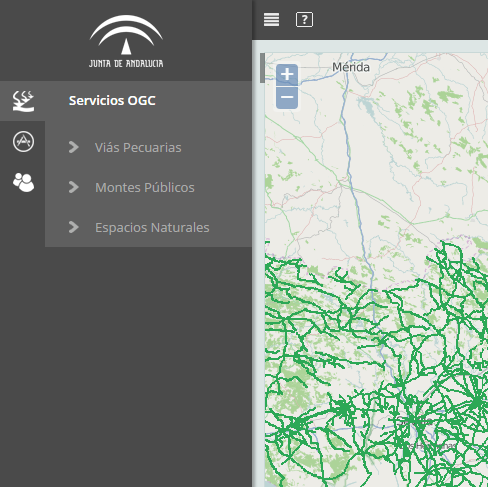
\includegraphics[width=\textwidth]{enia/seccion}
		\caption{Secci�n seleccionada.}
		\label{img_eniaSeccion}
	\end{minipage}
	~
	\begin{minipage}{0.49\textwidth}
		\centering
		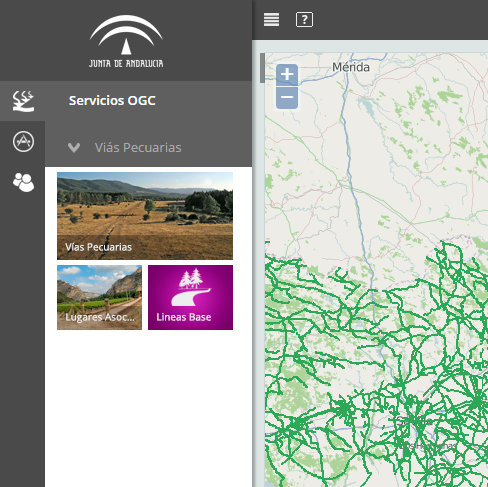
\includegraphics[width=\textwidth]{enia/subseccion}
		\caption{Subsecci�n seleccionada.}
		\label{img_eniaSubseccion}
	\end{minipage}
	
\end{figure}




%----------------------------------------------------------------------------------------
%	BIBLIOGRAPHY
%----------------------------------------------------------------------------------------

%\chapter*{Referencias}
%\addcontentsline{toc}{chapter}{\textcolor{ocre}{Referencias}}
\printbibliography
%\section*{Libros}
%\nocite{*}
%\addcontentsline{toc}{section}{Libros}
%\printbibliography[heading=bibempty,type=book]
%\section*{Art�culos}
%\nocite{*}
%\addcontentsline{toc}{section}{Art�culos}
%\printbibliography[heading=bibempty,type=article]
%\section*{Online}
%\nocite{*}
%\addcontentsline{toc}{section}{Online}
%\printbibliography[heading=bibempty,type=online]
%----------------------------------------------------------------------------------------
%	INDEX
%----------------------------------------------------------------------------------------

%\cleardoublepage
%\phantomsection
%\setlength{\columnsep}{0.75cm}
%\addcontentsline{toc}{chapter}{\textcolor{ocre}{Indice}}
%\printindex

%----------------------------------------------------------------------------------------

%----------------------------------------------------------------------------------------
% LAST PAGE
%----------------------------------------------------------------------------------------
%Anexo
\appendix
\chapter{Anexo}\label{anexo:I}
% Contenido del anexo I
% Table generated by Excel2LaTeX from sheet 'Hoja1'

Example of \url{https://es.overleaf.com/latex/examples/a-longtable-example/xxwzfxkxxjmc}.
\begin{center}
\begin{longtable}{|l|l|l|}
	\caption{A sample long table.} \label{tab:long} \\
	
	\hline \multicolumn{1}{|c|}{\textbf{First column}} & \multicolumn{1}{c|}{\textbf{Second column}} & \multicolumn{1}{c|}{\textbf{Third column}} \\ \hline 
	\endfirsthead
	
	\multicolumn{3}{c}%
	{{\bfseries \tablename\ \thetable{} -- continued from previous page}} \\
	\hline \multicolumn{1}{|c|}{\textbf{First column}} & \multicolumn{1}{c|}{\textbf{Second column}} & \multicolumn{1}{c|}{\textbf{Third column}} \\ \hline 
	\endhead
	
	\hline \multicolumn{3}{|r|}{{Continued on next page}} \\ \hline
	\endfoot
	
	\hline \hline
	\endlastfoot
	
	One & abcdef ghjijklmn & 123.456778 \\
	One & abcdef ghjijklmn & 123.456778 \\
	One & abcdef ghjijklmn & 123.456778 \\
	One & abcdef ghjijklmn & 123.456778 \\
	One & abcdef ghjijklmn & 123.456778 \\
	One & abcdef ghjijklmn & 123.456778 \\
	One & abcdef ghjijklmn & 123.456778 \\
	One & abcdef ghjijklmn & 123.456778 \\
	One & abcdef ghjijklmn & 123.456778 \\
	One & abcdef ghjijklmn & 123.456778 \\
	One & abcdef ghjijklmn & 123.456778 \\
	One & abcdef ghjijklmn & 123.456778 \\
	One & abcdef ghjijklmn & 123.456778 \\
	One & abcdef ghjijklmn & 123.456778 \\
	One & abcdef ghjijklmn & 123.456778 \\
	One & abcdef ghjijklmn & 123.456778 \\
	One & abcdef ghjijklmn & 123.456778 \\
	One & abcdef ghjijklmn & 123.456778 \\
	One & abcdef ghjijklmn & 123.456778 \\
	One & abcdef ghjijklmn & 123.456778 \\
	One & abcdef ghjijklmn & 123.456778 \\
	One & abcdef ghjijklmn & 123.456778 \\
	One & abcdef ghjijklmn & 123.456778 \\
	One & abcdef ghjijklmn & 123.456778 \\
	One & abcdef ghjijklmn & 123.456778 \\
	One & abcdef ghjijklmn & 123.456778 \\
	One & abcdef ghjijklmn & 123.456778 \\
	One & abcdef ghjijklmn & 123.456778 \\
	One & abcdef ghjijklmn & 123.456778 \\
	One & abcdef ghjijklmn & 123.456778 \\
	One & abcdef ghjijklmn & 123.456778 \\
	One & abcdef ghjijklmn & 123.456778 \\
	One & abcdef ghjijklmn & 123.456778 \\
	One & abcdef ghjijklmn & 123.456778 \\
	One & abcdef ghjijklmn & 123.456778 \\
	One & abcdef ghjijklmn & 123.456778 \\
	One & abcdef ghjijklmn & 123.456778 \\
	One & abcdef ghjijklmn & 123.456778 \\
	One & abcdef ghjijklmn & 123.456778 \\
	One & abcdef ghjijklmn & 123.456778 \\
	One & abcdef ghjijklmn & 123.456778 \\
	One & abcdef ghjijklmn & 123.456778 \\
	One & abcdef ghjijklmn & 123.456778 \\
	One & abcdef ghjijklmn & 123.456778 \\
	One & abcdef ghjijklmn & 123.456778 \\
	One & abcdef ghjijklmn & 123.456778 \\
	One & abcdef ghjijklmn & 123.456778 \\
	One & abcdef ghjijklmn & 123.456778 \\
	One & abcdef ghjijklmn & 123.456778 \\
	One & abcdef ghjijklmn & 123.456778 \\
	One & abcdef ghjijklmn & 123.456778 \\
	One & abcdef ghjijklmn & 123.456778 \\
	One & abcdef ghjijklmn & 123.456778 \\
	One & abcdef ghjijklmn & 123.456778 \\
	One & abcdef ghjijklmn & 123.456778 \\
	One & abcdef ghjijklmn & 123.456778 \\
	One & abcdef ghjijklmn & 123.456778 \\
	One & abcdef ghjijklmn & 123.456778 \\
	One & abcdef ghjijklmn & 123.456778 \\
	One & abcdef ghjijklmn & 123.456778 \\
	One & abcdef ghjijklmn & 123.456778 \\
	One & abcdef ghjijklmn & 123.456778 \\
	One & abcdef ghjijklmn & 123.456778 \\
	One & abcdef ghjijklmn & 123.456778 \\
	One & abcdef ghjijklmn & 123.456778 \\
	One & abcdef ghjijklmn & 123.456778 \\
	One & abcdef ghjijklmn & 123.456778 \\
	One & abcdef ghjijklmn & 123.456778 \\
	One & abcdef ghjijklmn & 123.456778 \\
	One & abcdef ghjijklmn & 123.456778 \\
	One & abcdef ghjijklmn & 123.456778 \\
	One & abcdef ghjijklmn & 123.456778 \\
	One & abcdef ghjijklmn & 123.456778 \\
	One & abcdef ghjijklmn & 123.456778 \\
	One & abcdef ghjijklmn & 123.456778 \\
	One & abcdef ghjijklmn & 123.456778 \\
	One & abcdef ghjijklmn & 123.456778 \\
	One & abcdef ghjijklmn & 123.456778 \\
	One & abcdef ghjijklmn & 123.456778 \\
	One & abcdef ghjijklmn & 123.456778 \\
\end{longtable}
\end{center}




\includepdf{TFG-back.pdf}

\end{document}